\documentclass{article}
\usepackage{amsmath} %This allows me to use the align functionality.
                     %If you find yourself trying to replicate
                     %something you found online, ensure you're
                     %loading the necessary packages!
\usepackage{amsfonts}%Math font
\usepackage{graphicx}%For including graphics
\usepackage{hyperref}%For Hyperlinks
\usepackage{natbib}        %For the bibliography
\bibliographystyle{apalike}%For the bibliography
\usepackage[margin=1.0in]{geometry}
\usepackage{float}
\usepackage{Sweave}
\begin{document}
\Sconcordance{concordance:HW0.tex:HW0.Rnw:%
1 12 1 1 0 31 1 1 7 6 0 1 1 6 0 2 2 1 0 1 2 1 0 1 1 3 0 1 2 5 1 1 5 4 0 %
1 7 5 0 1 16 14 0 1 9 7 0 1 3 1 0 1 1 1 6 4 0 1 2 1 0 1 1 1 3 6 0 1 1 6 %
0 1 2 11 1 1 2 4 0 1 2 14 1 1 3 2 0 2 1 1 7 6 0 2 1 1 4 2 0 1 1 1 7 6 0 %
2 1 1 3 6 0 1 1 6 0 1 2 11 1 1 2 1 0 2 1 1 19 17 0 1 1 6 0 1 2 13 1 1 2 %
7 0 2 1 1 2 7 0 1 1 5 0 1 1 5 0 1 1 5 0 1 1 6 0 1 2 5 1 1 9 8 0 2 1 1 %
13 12 0 1 1 3 0 1 2 1 3 2 0 1 1 1 15 17 0 1 2 1 3 2 0 9 1 3 0 1 2 29 1 %
6 0 1 5 16 1 1 3 8 0 2 1 1 3 7 0 1 3 1 0 1 13 14 0 1 2 1 8 1 2 2 1 1 5 %
4 0 1 2 1 0 1 1 4 0 1 3 1 5 1 2 1 10 1 2 3 1 15 0 1 14 1 1 7 0 1 6 1 1 %
23 0 1 22 1 1 24 0 1 23 1 1 10 0 1 9 29 1 1 2 1 0 2 1 18 0 1 2 7 0 1 1 %
1 2 1 0 1 1 1 2 1 0 1 2 4 0 1 2 51 1 1 6 4 0 1 2 1 0 2 1 5 0 3 1 5 0 1 %
1 19 0 1 12 11 0 1 1 19 0 1 3 2 0 1 1 5 0 1 3 2 0 1 1 5 0 1 11 10 0 1 1 %
19 0 2 1 5 0 2 1 5 0 1 15 14 0 1 1 19 0 2 1 5 0 2 1 5 0 1 15 14 0 1 1 %
19 0 2 1 5 0 2 1 5 0 1 15 14 0 1 1 19 0 2 1 5 0 2 1 21 0 1 15 1 1 4 0 1 %
3 2 1 1 7 1 2 1 7 1 2 1 7 1 2 1 7 1 2 1 7 1 2 1 7 1 2 1 7 1 2 1 7 1 2 1 %
7 1 2 1 7 1 2 2 1}

%set the size of the graphs to fit nicely on a 8.5x11 sheet
\noindent \textbf{MA 354: Data Analysis I -- Fall 2019}\\%\\ gives you a new line
\noindent \textbf{Homework 0: Alexa Canaan}\vspace{1em}\\
\emph{Complete the following opportunities to use what we've talked about in class. 
These questions will be graded for correctness, communication and succinctness. Ensure
you show your work and explain your logic in a legible and refined submission. If you
make a mistake while completing this assignment do not delete it -- instead, make a note
about why it's a mistake, how you realized it, and how you fixed it. The best, most 
productive recovery from a mistake will receive a 5 point bonus.}
%Comments -- anything after % is not put into the PDF
\begin{enumerate}
%%%%%%%%%%%%%%%%%%%%%%%%%%%%%%%%%%%%%%%%%%%%%%%%%%%%%%%%%%%%%%%%%%%%%%%%%%%%%%%
%%%%%%%%%%%%%%%%%%%%%%%%%%%%%%%%%%%%%%%%%%%%%%%%%%%%%%%%%%%%%%%%%%%%%%%%%%%%%%%
%%%%%%%%%  Question 0
%%%%%%%%%%%%%%%%%%%%%%%%%%%%%%%%%%%%%%%%%%%%%%%%%%%%%%%%%%%%%%%%%%%%%%%%%%%%%%%
%%%%%%%%%%%%%%%%%%%%%%%%%%%%%%%%%%%%%%%%%%%%%%%%%%%%%%%%%%%%%%%%%%%%%%%%%%%%%%%
  \item[0.] \textbf{Complete weekly diagnostics.} Upon completion of this assignment
  reflect, in a few sentences, on what you've learned since the beginning of the semester.
  Think about an mention any concepts you want or need to continue working on and
  list at least one goal for the next assignment.
%%%%%%%%%%%%%%%%%%%%%%%%%%%%%%%%%%%%%%%%%%%%%%%%%%%%%%%%%%%%%%%%%%%%%%%%%%%%%%%
%%%%%%%%%%%%%%%%%%%%%%%%%%%%%%%%%%%%%%%%%%%%%%%%%%%%%%%%%%%%%%%%%%%%%%%%%%%%%%%
%%%%%%%%%  Question 1
%%%%%%%%%%%%%%%%%%%%%%%%%%%%%%%%%%%%%%%%%%%%%%%%%%%%%%%%%%%%%%%%%%%%%%%%%%%%%%%
%%%%%%%%%%%%%%%%%%%%%%%%%%%%%%%%%%%%%%%%%%%%%%%%%%%%%%%%%%%%%%%%%%%%%%%%%%%%%%%
  \item \textbf{Writing Functions and Loops.} Create a function called \texttt{f1} 
  in \texttt{R}, in as few lines as possible that represents the  following function.
    \[f_1(x) = \ln\left(\sqrt{x*10^3}\right)\]
    Compare the runtime of your function to the one below using a loop that saves 
    the runtime of each function over 1000 iterations. Summarize and compare the results.
\begin{Schunk}
\begin{Sinput}
> f2 <- function(x){
+   a<- x*10^3
+   b<- sqrt(a)
+   c<- log(b)
+   return(c)
+ }
> f2(1)
\end{Sinput}
\begin{Soutput}
[1] 3.453878
\end{Soutput}
\end{Schunk}
You can track the runtime of code using the following \texttt{R} code.
\begin{Schunk}
\begin{Sinput}
> start_time <- Sys.time()
> #do things you want to time here
> end_time <- Sys.time()
> runtime <-end_time - start_time
\end{Sinput}
\end{Schunk}
You might want to report this runtime in your .pdf document, but you'll find that the 
runtime changes each time you compile your document. You can pass variable values in \texttt{R}
to the document using the \texttt{Sexpr} command. For example, the runtime of the comment above
is 0.001 seconds.

\textbf{Solution:}
\begin{Schunk}
\begin{Sinput}
> #creating f1 and f2 that perform the same function
> f1 <- function(x){ #my more efficient code
+   return(log(sqrt(x*10^3))) #originally put ln as a function here whoops
+   }
> f2 <- function(x){ #less efficient code
+   a<- x*10^3
+   b<- sqrt(a)
+   c<- log(b)
+   return(c)
+ }
> #test
> #start_time2 <- Sys.time()
> #f2(1)
> #end_time2 <- Sys.time()
> #runtime2 <- end_time1 - start_time2
> #runtime2
> 
> #runtime for f1
> r1 <- function(n){
+ start_time1 <- Sys.time() #start time
+ f1(1) #call efficient function
+ end_time1 <- Sys.time() #end time
+ runtime1 <-end_time1 - start_time1 #runtime
+ return(runtime1)
+ }
> #runtime for f2
> r2 <- function(n){
+ start_time2 <- Sys.time() #start time
+ f2(1) #call less efficient function
+ end_time2 <- Sys.time() #end time
+ runtime2 <-end_time2 - start_time2 #runtime
+ return(runtime2)
+ }
> #initialize 
> t1 = 0
> t2 = 0
> #1000 iterations of runtime for both functions
> for (number in 1:1000){ 
+   t1 = t1 + r1(1)
+   t2 = t2 + r2(1)
+ }
> #compare average difference of runtimes
> t1 = t1/1000
> t2 = t2/1000
> #output  
> t1
\end{Sinput}
\begin{Soutput}
Time difference of 7.054329e-06 secs
\end{Soutput}
\begin{Sinput}
> t2
\end{Sinput}
\begin{Soutput}
Time difference of 7.52902e-06 secs
\end{Soutput}
\end{Schunk}

The runtime for function 2 is greater than the runtime for function 1 because function 2 is creating variables which takes more runtime than simply using 1 variable. My program reported about a $3e^-06$ difference in runtimes as the average difference between the two functions.
\newpage
%%%%%%%%%%%%%%%%%%%%%%%%%%%%%%%%%%%%%%%%%%%%%%%%%%%%%%%%%%%%%%%%%%%%%%%%%%%%%%%
%%%%%%%%%%%%%%%%%%%%%%%%%%%%%%%%%%%%%%%%%%%%%%%%%%%%%%%%%%%%%%%%%%%%%%%%%%%%%%%
%%%%%%%%%  Question 2
%%%%%%%%%%%%%%%%%%%%%%%%%%%%%%%%%%%%%%%%%%%%%%%%%%%%%%%%%%%%%%%%%%%%%%%%%%%%%%%
%%%%%%%%%%%%%%%%%%%%%%%%%%%%%%%%%%%%%%%%%%%%%%%%%%%%%%%%%%%%%%%%%%%%%%%%%%%%%%%
  \item \textbf{Conditional Statements and Loops.} Assess which is faster.
  \begin{enumerate}
    \item Generate 1000 random integers between 1 and 1000 with replacement with
    the following \texttt{R} code.
\begin{Schunk}
\begin{Sinput}
> random.ints<-sample(x=1:1000,size=1000,replace=TRUE)
\end{Sinput}
\end{Schunk}
    Then, using a loop, create a vector named \texttt{random.type} that is ``odd"
    when the corresponding value in \texttt{random.ints} is odd and ``even" otherwise.
    \begin{enumerate}
      \item Add elements to the vector called \texttt{random.type} as they
      are decided; e.g., for an iteration where the value is odd we add
      an element using \texttt{random.type<-c(random.type,"odd")}.
      \item Create an empty vector of size 1000 (with \texttt{NA} entries) to 
      start and place elements into the vector; e.g., for iteration $i$
      where the value is odd we place the element using \texttt{random.type[i]}.
    \end{enumerate}
    Which is faster?
\end{enumerate}

\textbf{Solution:}
Part 2 is faster. Placing elements into a vector is faster than creating them and then placing them in the vector.
\begin{Schunk}
\begin{Sinput}
> #part i - add elements to a vector as they are decided
> random.ints1 <-sample(x=1:1000,size=1000,replace=TRUE)
> start_timei <- Sys.time() #time the process
> random.type1 <- c()
> for (i in 1:1000){
+   if (random.ints1[i]%%2 != 0) { #iterate through each value
+     random.type1<- c(random.type1,"odd")
+   } else {
+     random.type1<- c(random.type1,"even")
+   }
+ }
> end_timei <- Sys.time()
> runtimei <-end_timei - start_timei
> #part ii - create a vector and then place elements into vector
> #random.ints<-sample(x=1:1000,size=1000,replace=TRUE)
> start_timeii <- Sys.time() #time the process
> random.type = rep(NA, 1000)
> for (i in 1:1000){
+   if (random.ints1[1]%%2 != 0){
+     vec <- c(random.type[i],"odd")
+   } else {
+     vec <- c(random.type[i], "even")
+   }
+ }
> end_timeii <- Sys.time()
> runtimeii <-end_timeii - start_timeii
> #output and compare the start time and end time
> print(runtimei)
\end{Sinput}
\begin{Soutput}
Time difference of 0.01355505 secs
\end{Soutput}
\begin{Sinput}
> print(runtimeii)
\end{Sinput}
\begin{Soutput}
Time difference of 0.009389877 secs
\end{Soutput}
\end{Schunk}
\newpage
%%%%%%%%%%%%%%%%%%%%%%%%%%%%%%%%%%%%%%%%%%%%%%%%%%%%%%%%%%%%%%%%%%%%%%%%%%%%%%%
%%%%%%%%%%%%%%%%%%%%%%%%%%%%%%%%%%%%%%%%%%%%%%%%%%%%%%%%%%%%%%%%%%%%%%%%%%%%%%%
%%%%%%%%%  Question 3
%%%%%%%%%%%%%%%%%%%%%%%%%%%%%%%%%%%%%%%%%%%%%%%%%%%%%%%%%%%%%%%%%%%%%%%%%%%%%%%
%%%%%%%%%%%%%%%%%%%%%%%%%%%%%%%%%%%%%%%%%%%%%%%%%%%%%%%%%%%%%%%%%%%%%%%%%%%%%%%
  \item \textbf{Conditional Statements and Loops} Each new term in the Fibonacci sequence is 
  generated by adding the previous two terms. By starting with 1 and 2, the first 
  10 terms will be 1, 2, 3, 5, 8, 13, 21, 34, 55, 89. Find the sum of the even terms in the 
  Fibonacci sequence whose values do not exceed one million.

\textbf{Solution:}  
\begin{Schunk}
\begin{Sinput}
> num1 = 1 #first term
> num2 = 2 #second term
> sums = 0 #initialize sum
> while (num1 <= 1000000 & num2 <= 1000000){ #must be under 1000000
+   newnum = num1 + num2 #creating next variable in sequence
+   #misunderstood the question here, thought I was trying to add up the sum closest to, but not exceeding one million
+    # if (newnum + sums > 1000000){
+    #   break - I tried to break which ended up not working as well and wasn't good coding practice
+    # }
+    if (newnum%%2==0){ #checks it's an even number
+      sums = sums + newnum #creates a new number for the sequence
+    } 
+    # else {
+    #   print(sums)
+    # }
+    if (num1<num2){ #adds the new number to the sequence
+      num1 = newnum 
+    } else {
+      num2 = newnum
+    }
+  }
>  sums #answer
\end{Sinput}
\begin{Soutput}
[1] 1089152
\end{Soutput}
\end{Schunk}
\newpage
%%%%%%%%%%%%%%%%%%%%%%%%%%%%%%%%%%%%%%%%%%%%%%%%%%%%%%%%%%%%%%%%%%%%%%%%%%%%%%%
%%%%%%%%%%%%%%%%%%%%%%%%%%%%%%%%%%%%%%%%%%%%%%%%%%%%%%%%%%%%%%%%%%%%%%%%%%%%%%%
%%%%%%%%%  Question 4
%%%%%%%%%%%%%%%%%%%%%%%%%%%%%%%%%%%%%%%%%%%%%%%%%%%%%%%%%%%%%%%%%%%%%%%%%%%%%%%
%%%%%%%%%%%%%%%%%%%%%%%%%%%%%%%%%%%%%%%%%%%%%%%%%%%%%%%%%%%%%%%%%%%%%%%%%%%%%%%  
  \item  \textbf{Conditional Statements and Loops} A palindromic number reads the same 
  both ways. The largest palindrome made from the product of two 2-digit numbers is 
  $9009 = 91 \times 99$. Find the largest palindrome made from the product of two 3-digit numbers.
  
  You can get the reverse of a number using the ``stringr" package for \texttt{R}
  (practice Sweave by putting by the citation here:
  \cite{R}) as follows.
 
\begin{Schunk}
\begin{Sinput}
> install.packages("stringr",repos = "https://cloud.r-project.org")
\end{Sinput}
\begin{Soutput}
The downloaded binary packages are in
	/var/folders/7b/05g8dtkd3cb4hf1p73knpz1w0000gn/T//RtmpE9LdyJ/downloaded_packages
\end{Soutput}
\begin{Sinput}
> library(stringr)
> number.to.reverse <- 1234
> #creates a list containing a vector of characters
> (split.number<-str_split(number.to.reverse,pattern=""))
\end{Sinput}
\begin{Soutput}
[[1]]
[1] "1" "2" "3" "4"
\end{Soutput}
\begin{Sinput}
> (split.number<-split.number[[1]]) #takes just the vector
\end{Sinput}
\begin{Soutput}
[1] "1" "2" "3" "4"
\end{Soutput}
\begin{Sinput}
> (split.number.reversed <- rev(split.number)) #reverses the order of the vector
\end{Sinput}
\begin{Soutput}
[1] "4" "3" "2" "1"
\end{Soutput}
\begin{Sinput}
> (reversed.number <- paste(split.number.reversed, collapse="")) #paste items back together
\end{Sinput}
\begin{Soutput}
[1] "4321"
\end{Soutput}
\begin{Sinput}
> (reversed.number<-as.numeric(reversed.number)) #treat it like a number
\end{Sinput}
\begin{Soutput}
[1] 4321
\end{Soutput}
\end{Schunk}
\textbf{Remark:} You'll find that the solution to this question will elongate the
compiling time for the .pdf. That's okay. Once you're happy with the solution 
you can type the output into your code chunk and set eval=FALSE between the left
and right arrows.

\textbf{Solution:}  
\begin{Schunk}
\begin{Sinput}
> # the way I originally thought of this problem, 
> #I was trying to break out of the nested for loop. 
> #After taking a break and coming back to the problem, 
> #I recognize that if I store the maximum variable 
> #and replace it only when finding a greater palindrome, 
> #I would be able to find the answer. 
> #This takes more time to compile, but does get me the right answer
> install.packages("stringr",repos = "https://cloud.r-project.org")
> library(stringr)
> maxnum = 0
> for (num1 in 999:100){ #double loop to hit every possible pair
+   for (num2 in 999:100){
+     pp = num1 * num2 #find the product
+     split.number<-str_split(pp,pattern="")
+     split.number<-split.number[[1]]
+     split.number.reversed <- rev(split.number) #reverses the order of the vector
+     reversed.number <- paste(split.number.reversed, collapse="")   #paste items back together
+     reversed.number<-as.numeric(reversed.number) #treat it like a number
+     if (pp == reversed.number & pp > maxnum){ #decide if the number  is the largest palindrome found thus far
+       maxnum = pp 
+       }
+   }
+ }
> print(maxnum)
\end{Sinput}
\end{Schunk}

\begin{Schunk}
\begin{Sinput}
> #other attempt
> install.packages("stringr",repos = "https://cloud.r-project.org")
> library(stringr)
> for (num in 999:100){ #create the product using 3 digit numbers, only changing one number but this way actually decreases both numbers at the same time
+   num1 = 999
+   pp = num1 * num 
+   split.number<-str_split(pp,pattern="")
+   split.number<-split.number[[1]]
+   split.number.reversed <- rev(split.number) #reverses the order of the vector
+   reversed.number <- paste(split.number.reversed, collapse="")   #paste items back together
+   reversed.number<-as.numeric(reversed.number) #treat it like a number
+   if (pp == reversed.number){
+     print(pp)
+     break
+   } else {
+     num1 = num1 - 1
+   }
+ }
\end{Sinput}
\end{Schunk}

\begin{Schunk}
\begin{Sinput}
> #other attempt
> install.packages("stringr",repos = "https://cloud.r-project.org")
> library(stringr)
> num1 = 999 #not as efficient as creating a for loop
> num2 = 999
> pp = num1 * num2 
> split.number<-str_split(pp,pattern="")
> split.number<-split.number[[1]]
> split.number.reversed <- rev(split.number) #reverses the order of the vector
> reversed.number <- paste(split.number.reversed, collapse="")   #paste items back together
> reversed.number<-as.numeric(reversed.number) #treat it like a number
\end{Sinput}
\end{Schunk}
\newpage
%%%%%%%%%%%%%%%%%%%%%%%%%%%%%%%%%%%%%%%%%%%%%%%%%%%%%%%%%%%%%%%%%%%%%%%%%%%%%%%
%%%%%%%%%%%%%%%%%%%%%%%%%%%%%%%%%%%%%%%%%%%%%%%%%%%%%%%%%%%%%%%%%%%%%%%%%%%%%%%
%%%%%%%%%  Question 5
%%%%%%%%%%%%%%%%%%%%%%%%%%%%%%%%%%%%%%%%%%%%%%%%%%%%%%%%%%%%%%%%%%%%%%%%%%%%%%%
%%%%%%%%%%%%%%%%%%%%%%%%%%%%%%%%%%%%%%%%%%%%%%%%%%%%%%%%%%%%%%%%%%%%%%%%%%%%%%%
  \item \textbf{(Working with Data)} Below you will load and summarize a dataset 
  containing 575 observations of drug treatments. The data includes the following
  \begin{itemize}
    \item ID --	Identification Code	(1 - 575)
    \item AGE	-- Age at Enrollment	(Years)
    \item BECK -- Beck Depression Score	(0.000 - 54.000)
    \item HC --	Heroin/Cocaine Use During	3 Months Prior to Admission (1 = Heroin
    \& Cocaine; 2 = Heroin Only, 3 = Cocaine Only; 4 = Neither Heroin nor Cocaine)
    \item IV -- History of IV Drug Use	(1 = Never; 2 = Previous; 3 = Recent)
    \item IV3	-- Recent IV use	(1 = Yes; 0 = No)
    \item NDT -- Number of Prior Drug Treatments (0 - 40)
    \item RACE -- Subject's Race	(0 = White; 1 = Non-White)
    \item TREAT -- Treatment Randomization (0 = Short Assignment;	1 = Long Assignment)
    \item SITE -- Treatment Site (0 = A; 1 = B)
    \item LEN.T	-- Length of Stay in Treatment (Days Admission Date to Exit Date)	
    \item TIME -- Time to Drug Relapse (Days Measured from Admission Date)
    \item CENSOR -- Event for Treating Lost to Follow-Up as Returned to Drugs 
    (1 = Returned to Drugs or Lost to Follow-Up; 0 = Otherwise)
    \item etc.
  \end{itemize}
  \begin{enumerate} %this begins a lettered enumerate so I can ask more 
                    %than one question in a question.
    \item Load the data provided in the ``quantreg" package for \texttt{R} \citep{quantreg}.
\begin{Schunk}
\begin{Sinput}
> # install.packages("quantreg",repos = "http://cloud.r-project.org/")
> # library("quantreg")
> # data("uis")
\end{Sinput}
\end{Schunk}

    \item Numerically summarize the Beck Depression Score of the observed drug 
    treatment patients. Note the following designations of the test when interpreting
    your results.
    \begin{itemize}
      \item 0-13: minimal depression
      \item 14-19: mild depression
      \item 20-28: moderate depression
      \item 29-63: severe depression.
    \end{itemize}
    \item Graphically summarize the Beck Depression Score of the
    observed drug treatment patients. Interpret the results through 
    the lens of the scale above.
    \item List three questions about drug use that we might be able to answer based on the 
    data we have.
  \end{enumerate}
\textbf{Solution:}
\begin{Schunk}
\begin{Sinput}
> #PART A: Load the data
> install.packages("quantreg",repos = "http://cloud.r-project.org/")
\end{Sinput}
\begin{Soutput}
The downloaded binary packages are in
	/var/folders/7b/05g8dtkd3cb4hf1p73knpz1w0000gn/T//RtmpE9LdyJ/downloaded_packages
\end{Soutput}
\begin{Sinput}
> library("quantreg")
> data("uis")
> #PART B: Summarize the data
> summary(uis$BECK)
\end{Sinput}
\begin{Soutput}
   Min. 1st Qu.  Median    Mean 3rd Qu.    Max. 
   0.00   10.00   17.00   17.37   23.00   54.00 
\end{Soutput}
\begin{Sinput}
> #create counts of designations of depression from mild to severe 
> uis["depression.severity"]<-NA
> #creates a degree designation for each observation
> for (i in 1:575) {
+   if (uis$BECK[i] >= 0 & uis$BECK[i] <= 13) {
+     uis$depression.severity[i] = "minimal"
+   } else if (uis$BECK[i] > 13 & uis$BECK[i] <= 19) {
+     uis$depression.severity[i] = "mild"
+   } else if (uis$BECK[i] > 19 & uis$BECK[i] <= 28) {
+     uis$depression.severity[i] = "moderate"
+   } else if (uis$BECK[i] > 28 & uis$BECK[i] <= 63) {
+     uis$depression.severity[i] = "severe"
+   }
+ }
\end{Sinput}
\end{Schunk}

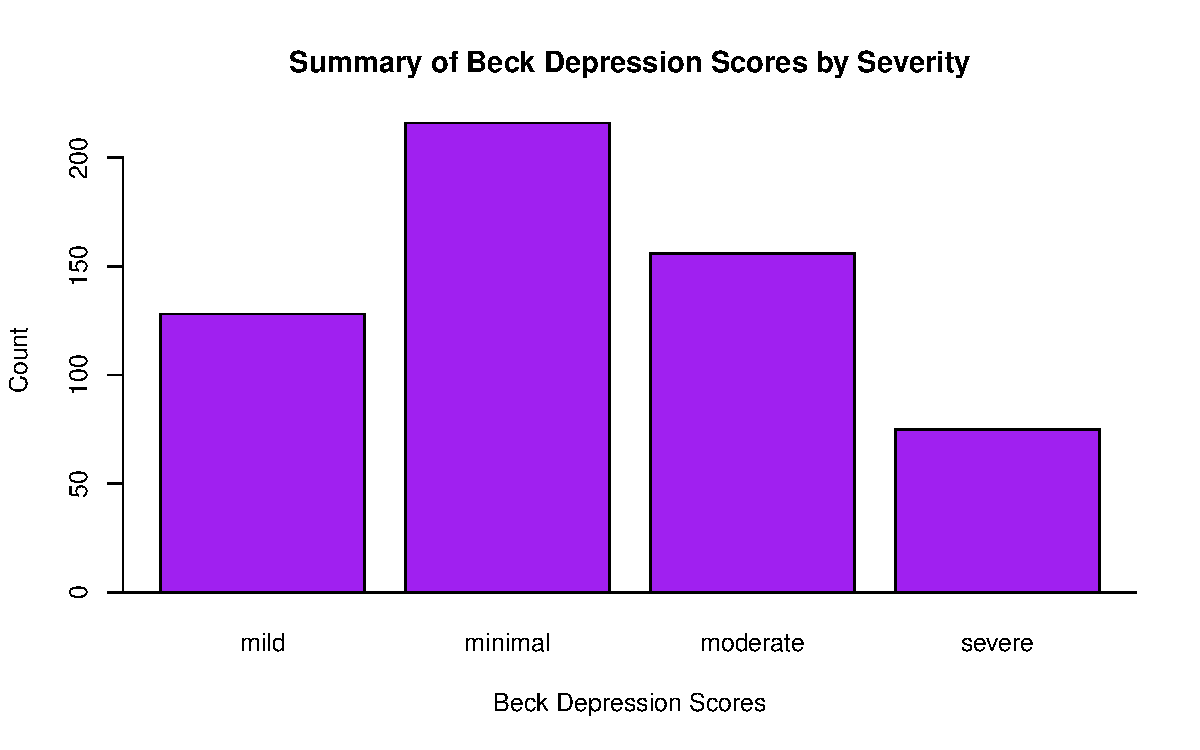
\includegraphics{HW0-013}

As is seen in the figure, Beck Depression Scores seem to be right skewed in terms of severity. It seems like the most people are minimally depressed (200+), while around 80 people are severely depressed, the smallest category. The median depression score is 17 and the mean is 17.37, meaning that the data doesn't seem to be too skewed. The maximum depression score is 54 and the minimum depression score is 0.

\begin{Schunk}
\begin{Sinput}
> #PART C: Graphically summarize the BDS
> #install appropriate packages
> #install.packages("ggplot2")
> library(ggplot2)
> #install.packages("graphics")
> library(graphics)
> library(gridExtra)
> 
\end{Sinput}
\end{Schunk}

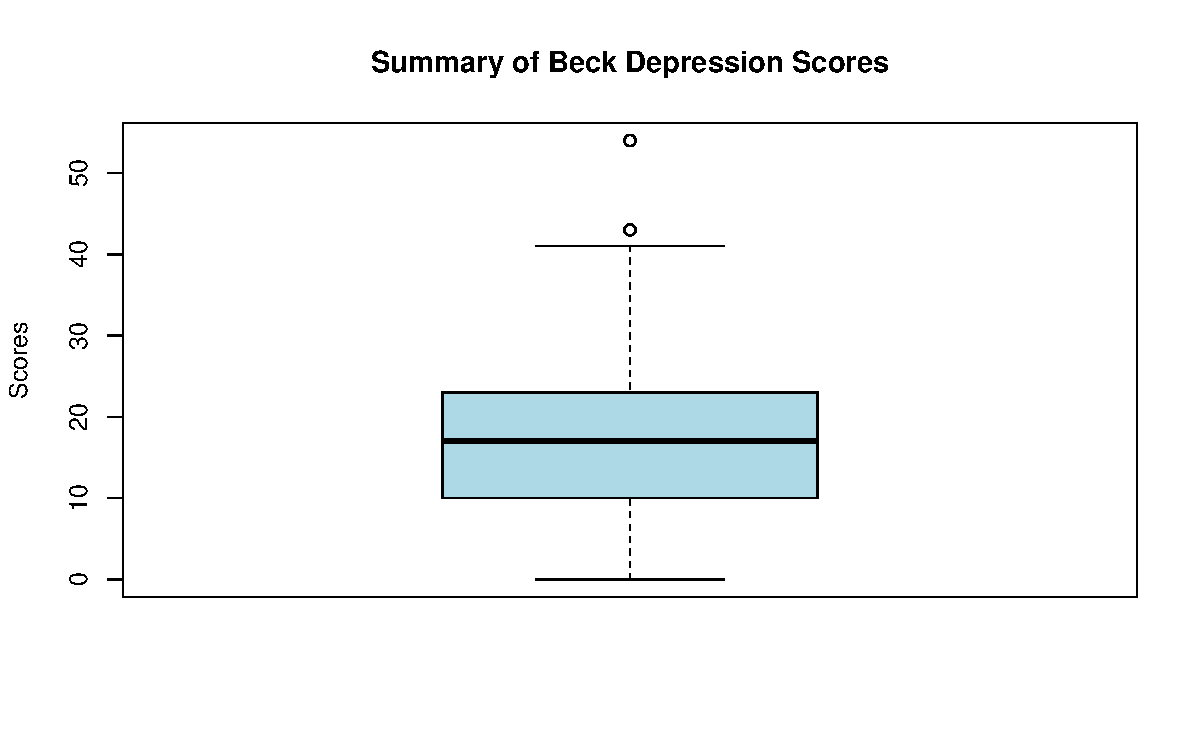
\includegraphics{HW0-015}

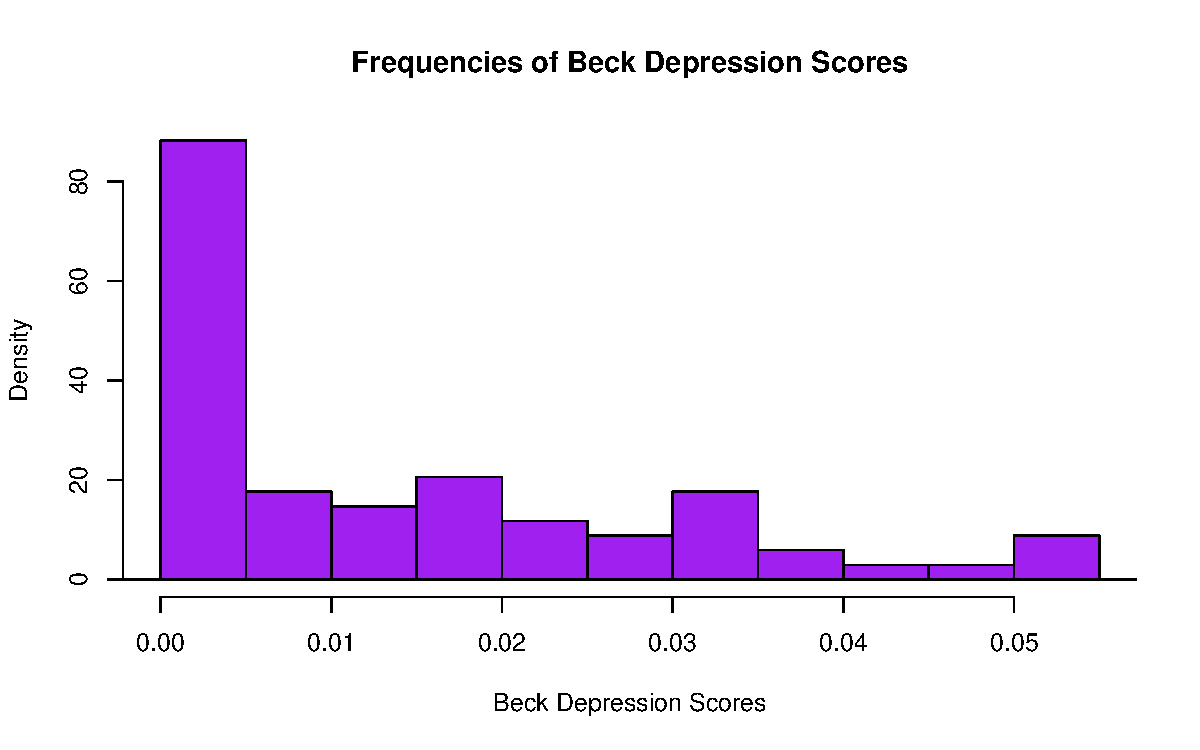
\includegraphics{HW0-016}

The boxplot indicates to us that half of the depression scores in the sample are between 10 and 23, meaning that half of the sample is between mnimally and moderately depressed. 75 percent of the scores in the sample are 23 or lower, meaning that most people are moderately depressed or less depressed.While the maximum depression score in this sample is 54, that score along with the score above 40 are both outliers, which may be causing the right skew and explain why the range of scores for severe depression is so large. When looking at the histogram below, we see that most depression scores are concentrated in the range of minimally depressed, with the first spike being the largest by 0.00. We see a relatively taller bar at the right end of the histogram compared to the two bars to the left of it which further illustrates that there are two outliers in the data under the severely depressed category. 

\begin{Schunk}
\begin{Sinput}
> #Plot2
> # dataframe2<-data.frame(prop.table(table(uis$BECK)))
> # p2<-ggplot(data=dataframe2, aes(x="Var1", y="Freq")) +
> #   geom_bar(stat= "identity",
> #            color= "black",
> #            fill= "lightblue") +
> #   xlab("Beck Depression Score") +
> #   ylab("Proportion") +
> #   ggtitle("Relative Frequencies of Beck Depression Scores of Drug Treatment Patients") +
> #   geom_hline(yintercept=0)
> #   theme_bw()
> # p2
\end{Sinput}
\end{Schunk}

\begin{Schunk}
\begin{Sinput}
> #Questions to consider, given the data
> #1. Does age of enrollment of the patient have an effect on time to drug relapse? (regression)
> #2. Does time to drug relapse vary by treatment randomization?
> #3. Is time to drug relapse correlated with the use or non-use of herion and/or cocaine during the 3 months prior to Admission?
\end{Sinput}
\end{Schunk}

\begin{Schunk}
\begin{Sinput}
> # par(mfrow=c(1,2)) #graphics settings 1 row, 2 columns of plots
> # #Frequency barplot
> # barplot(table(uis$BECK),
> #   main="Frequencies of Beck Depression Scores of Drug Treatment Patients",
> #   xlab="Beck Depression Scores", 
> #   ylab="Frequency",
> #   col="lightblue")
> #   abline(h=0)
> # 
> # #Relative Frequency Bar Plot
> # barplot(prop.table(table(uis$depressionlevel)),
> #   main="Frequencies of Beck Depression Scores of Drug Treatment Patients",
> #   xlab="Beck Depression Scores", ylab="Relative Frequency",
> #   col="lightblue")
> #   abline(h=0)
> #   
> # boxplot(uis$BECK)
> #   main="Beck Depression Scores"
> #   xlab=""
> #   ylab="Frequency"
\end{Sinput}
\end{Schunk}
  
\begin{Schunk}
\begin{Sinput}
> #my computer was getting mad when compiling the PDF
> #and I used ggplot, so I decided to make normal plots instead :(
> # <<p1,fig=TRUE,eval=TRUE>>=
> # #Plot1
> # dataframe<-data.frame(table(uis$BECK))
> # colnames(dataframe)=c("BDS","Freq")
> # p1<-ggplot(dataframe, aes(x=BDS, y=Freq)) +
> #   geom_boxplot(fill="lightblue") +
> #   xlab("Beck Depression Score") +
> #   ylab("Count") +
> #   ggtitle("Frequencies of Beck Depression Scores of Drug Treatment Patients") +
> #   theme_bw()
> # p1
> # @
> # \begin{figure}[H]
> # \centering 
> # <<p1,echo=FALSE>>=
> # @
> # \caption{hi}
> # \end{figure}
> 
\end{Sinput}
\end{Schunk}

\begin{Schunk}
\begin{Sinput}
> #Frequency barplot
> # barplot(table(uis$BECK),
> #   main="Frequencies of Beck Depression Scores of Drug Treatment Patients",
> #   xlab="Beck Depression Scores", 
> #   ylab="Frequency",
> #   col="lightblue")
> #   abline(h=0)
\end{Sinput}
\end{Schunk}

\newpage
  %%%%%%%%%%%%%%%%%%%%%%%%%%%%%%%%%%%%%%%%%%%%%%%%%%%%%%%%%%%%%%%%%%%%%%%%%%%%%%%
  %%%%%%%%%%%%%%%%%%%%%%%%%%%%%%%%%%%%%%%%%%%%%%%%%%%%%%%%%%%%%%%%%%%%%%%%%%%%%%%
  %%%%%%%%%  Question 6
  %%%%%%%%%%%%%%%%%%%%%%%%%%%%%%%%%%%%%%%%%%%%%%%%%%%%%%%%%%%%%%%%%%%%%%%%%%%%%%%
  %%%%%%%%%%%%%%%%%%%%%%%%%%%%%%%%%%%%%%%%%%%%%%%%%%%%%%%%%%%%%%%%%%%%%%%%%%%%%%%
    \item \textbf{(Working with Data)} Hepatitis C is a disease 
    that affects the liver. The virus that causes hepatitis C 
    is spread through blood or bodily fluids of an infected person. 
    The virus is often difficult to diagnose because there are few unique 
    symptoms. Those infected, however, sometimes experience jaundice -- a 
    condition that causes yellowing of the skin or eyes, as the liver 
    is infected.

    \cite{Bracht16} consider the human microfibrillar-associated protein 4,
    or MFAP4, and its role in disease-related tissue. Stage 0--no fibrosis; 
    Stage 1--enlarged, fibrotic portal tracts; Stage 2--periportal fibrosis 
    or portal-portal septa, but intact architecture; Stage 3--fibrosis with
    architectural distortion, but no obvious cirrhosis; and Stage 4--probable
    or definite cirrhosis.

    Previously, it has been shown that MFAP4 is a biomarker candidate for hepatic
    fibrosis and cirrhosis in hepatitis C patients. The analysis of \cite{Bracht16}
    aimed to consider the ability of MFAP4 to differentiate between stages of the 
    disease -- fibrosis stages (0-2) and cirrhosis (3-4) based on the Scheuer 
    scoring system.
    
    Below, I load the data and calculate the age of patients using the ``lubridate"
    package for \texttt{R} \citep{lubridate}.
\begin{Schunk}
\begin{Sinput}
> fn<-"http://cipolli.com/students/data/biomarker.csv"
> dat <- read.csv(file=fn, header=TRUE, sep=",")
> head(dat)
\end{Sinput}
\begin{Soutput}
  Patient.ID Year.of.Birth Gender Date.of.sampling Fibrosis.Stage HCV.Genotype
1       1112          1958 female         2/1/2005              0            1
2       3403          1946 female        1/18/2005              2             
3       2841          1954 female         1/3/2005              3            1
4        654          1958   male         2/1/2005              3            1
5       2788          1960   male        12/9/2004              0            3
6       2242          1954 female        5/12/2004              0            1
  MFAP4.U.mL
1        5.1
2        5.3
3       12.9
4        6.2
5        3.3
6        7.5
\end{Soutput}
\begin{Sinput}
> ###Calculate the age of each subject
> install.packages("lubridate",repos = "http://cloud.r-project.org/")
\end{Sinput}
\begin{Soutput}
The downloaded binary packages are in
	/var/folders/7b/05g8dtkd3cb4hf1p73knpz1w0000gn/T//RtmpE9LdyJ/downloaded_packages
\end{Soutput}
\begin{Sinput}
> library(lubridate)
> ###Create Date Variable for Date Sampled
> dos<-mdy(dat$Date.of.sampling)
> dos.year<-year(dos)
> ###Create age Variable
> age <- dos.year - dat$Year.of.Birth
> ###Add age to original dataset
> dat<-data.frame(dat,age)
\end{Sinput}
\end{Schunk}
  \begin{enumerate}
  \item Recreate Table 1 in \href{the paper}{https://www.ncbi.nlm.nih.gov/pmc/articles/PMC4932744/}. 
  Add a row to this table labeled ``Median age IQR." I've provided the LaTeX code for the
  table and made the first entry so you can see how it works.

\begin{table}[H]
  \centering
    \begin{tabular}{lccccccc}\hline
    Fibrosis Stage    & F0 & F1 & F2 & F3 & F4 & All\\\hline\hline
    \textbf{Age}                &&&&&&\\
    Mean age SD        &$43.75 \pm 12.11$ & $44.83 \pm 12.64$ & $51.24 \pm 12.04$  & $57.10 \pm 10.4$
                                & $57.33 \pm 11.31$        
                                &  $49.3 \pm 13.08$      \\
    Median age IQR     &  $45(16)$      &  $46(17.5)$       & $51(19)$
                                &  $57(14.5)$      & $56(16.5)$
                                &  $49(18)$      \\
    \textbf{Gender}             &&&&&&\\
    Women              &  $52$     & $85$       & $66$
                                &  $36$      & $28$
                                &  $267$      \\
    Men                &  $45$      & $91$       & $69$
                                &  $31$      & $39$
                                &  $275$      \\
    Number of patients &  $97$      &  $176$      & $135$
                                & $67$       & $67$
                                & $542$       \\
    \textbf{HCV genotype}       &&&&&&\\
    1                  &  $70$      & $126$       & $100$
                                &  $50$      & $43$
                                &  $389$     \\
    2                  &  $2$      & $12$       & $1$
                                &  $1$      & $3$
                                &  $19$      \\
    3                  &  $11$      & $25$       & $12$
                                &  $5$      & $7$
                                &  $60$      \\
    4                  &  $0$      &  $4$      & $4$
                                &  $1$      & $0$
                                &  $9$      \\
    Other              &  $0$      & $1$       & $0$
                                & $0$       & $0$
                                &  $1$      \\
    NA                 &  $14$      & $8$       & $18$
                                &  $10$      & $14$
                                &  $64$      \\\hline
    \end{tabular}
    \caption{Patient cohorts characteristics, subdivided by fibrosis stage}
  \end{table}
  \item Create several graphs that may be helpful for the researchers.
  \end{enumerate}
\end{enumerate}
\textbf{Solution:}
\begin{Schunk}
\begin{Sinput}
> #FIND VALUES FOR TABLE
> #installed dplyr: data manipulation package
> #install.packages("dplyr")
> library(dplyr)
> #all
> meanage_all= mean(dat$age)
> sdage_all= sd(dat$age)
> sdage_all
\end{Sinput}
\begin{Soutput}
[1] 13.08264
\end{Soutput}
\begin{Sinput}
> medianage_all= median(dat$age)
> medianIQRage_all= IQR(dat$age)
> medianIQRage_all
\end{Sinput}
\begin{Soutput}
[1] 18
\end{Soutput}
\begin{Sinput}
> summary(dat) #counts for the all columns 
\end{Sinput}
\begin{Soutput}
   Patient.ID   Year.of.Birth     Gender     Date.of.sampling Fibrosis.Stage 
 Min.   :   2   Min.   :1922   female:267   1/19/2004:  5     Min.   :0.000  
 1st Qu.:1074   1st Qu.:1946   male  :275   1/20/2004:  5     1st Qu.:1.000  
 Median :1952   Median :1955                1/6/2004 :  5     Median :1.000  
 Mean   :1949   Mean   :1955                3/9/2004 :  5     Mean   :1.688  
 3rd Qu.:2874   3rd Qu.:1963                9/13/2005:  5     3rd Qu.:2.000  
 Max.   :3772   Max.   :1993                9/8/2005 :  5     Max.   :4.000  
                                            (Other)  :512                    
 HCV.Genotype   MFAP4.U.mL         age      
       : 64   Min.   : 2.10   Min.   :12.0  
 1     :389   1st Qu.: 6.40   1st Qu.:41.0  
 2     : 19   Median : 9.75   Median :49.0  
 3     : 60   Mean   :13.79   Mean   :49.3  
 4     :  9   3rd Qu.:16.88   3rd Qu.:59.0  
 andere:  1   Max.   :94.20   Max.   :84.0  
\end{Soutput}
\begin{Sinput}
> #female: 267
> #male: 275
> #number of patients: 542
> #HCV 1: 389
> #HCV 2: 19
> #HCV 3: 60
> #HCV 4: 9
> #HCV Other(andere for the dutch): 1
> #HCV NA: 64
> 
> #created filtered dataframes for each stage of fibrosis and then found the summary statistics to fill in the table
> dat.fil0=filter(dat, Fibrosis.Stage==0) 
> summary(dat.fil0)
\end{Sinput}
\begin{Soutput}
   Patient.ID   Year.of.Birth     Gender     Date.of.sampling Fibrosis.Stage
 Min.   :  13   Min.   :1933   female:52   1/16/2006 : 3      Min.   :0     
 1st Qu.:1182   1st Qu.:1953   male  :45   12/17/2003: 2      1st Qu.:0     
 Median :1934   Median :1960               2/19/2004 : 2      Median :0     
 Mean   :2000   Mean   :1961               2/6/2006  : 2      Mean   :0     
 3rd Qu.:2907   3rd Qu.:1969               5/12/2004 : 2      3rd Qu.:0     
 Max.   :3675   Max.   :1988               7/27/2005 : 2      Max.   :0     
                                           (Other)   :84                    
 HCV.Genotype   MFAP4.U.mL         age       
       :14    Min.   : 2.10   Min.   :16.00  
 1     :70    1st Qu.: 5.00   1st Qu.:35.00  
 2     : 2    Median : 7.50   Median :45.00  
 3     :11    Mean   : 9.23   Mean   :43.75  
 4     : 0    3rd Qu.:10.90   3rd Qu.:51.00  
 andere: 0    Max.   :39.40   Max.   :71.00  
\end{Soutput}
\begin{Sinput}
> #meanage0: 43.75
> #sdage0: FIND
> sdage0= sd(dat.fil0$age)
> sdage0
\end{Sinput}
\begin{Soutput}
[1] 12.11407
\end{Soutput}
\begin{Sinput}
> #medianage0: 45
> #IQRage0: FIND
> IQRage0= IQR(dat.fil0$age)
> IQRage0
\end{Sinput}
\begin{Soutput}
[1] 16
\end{Soutput}
\begin{Sinput}
> #female: 52
> #male: 45
> #number of patients: 97
> #HCV 1: 70
> #HCV 2: 2
> #HCV 3: 11
> #HCV 4: 0 
> #HCV Other: 0
> #HCV NA: 14
> 
> dat.fil1=filter(dat, Fibrosis.Stage==1)
> summary(dat.fil1)
\end{Sinput}
\begin{Soutput}
   Patient.ID   Year.of.Birth     Gender     Date.of.sampling Fibrosis.Stage
 Min.   :   2   Min.   :1930   female:85   11/11/2003:  3     Min.   :1     
 1st Qu.:1128   1st Qu.:1951   male  :91   12/8/2003 :  3     1st Qu.:1     
 Median :2170   Median :1959               5/10/2004 :  3     Median :1     
 Mean   :2047   Mean   :1960               9/13/2005 :  3     Mean   :1     
 3rd Qu.:2990   3rd Qu.:1969               9/8/2005  :  3     3rd Qu.:1     
 Max.   :3752   Max.   :1992               10/18/2005:  2     Max.   :1     
                                           (Other)   :159                   
 HCV.Genotype   MFAP4.U.mL          age       
       :  8   Min.   : 2.300   Min.   :12.00  
 1     :126   1st Qu.: 5.775   1st Qu.:35.75  
 2     : 12   Median : 8.300   Median :46.00  
 3     : 25   Mean   :10.531   Mean   :44.83  
 4     :  4   3rd Qu.:12.125   3rd Qu.:53.25  
 andere:  1   Max.   :61.100   Max.   :74.00  
\end{Soutput}
\begin{Sinput}
> sdage1= sd(dat.fil1$age)
> sdage1
\end{Sinput}
\begin{Soutput}
[1] 12.64298
\end{Soutput}
\begin{Sinput}
> IQRage1= IQR(dat.fil1$age)
> IQRage1
\end{Sinput}
\begin{Soutput}
[1] 17.5
\end{Soutput}
\begin{Sinput}
> #meanage1: 44.83
> #sdage1: FIND
> #medianage1: 46
> #IQRage1: FIND
> #female: 85
> #male: 91
> #number of patients:176
> #HCV 1: 126
> #HCV 2: 12
> #HCV 3: 25
> #HCV 4: 4
> #HCV Other: 1
> #HCV NA: 8
> 
> dat.fil2=filter(dat, Fibrosis.Stage==2)
> summary(dat.fil2)
\end{Sinput}
\begin{Soutput}
   Patient.ID   Year.of.Birth     Gender     Date.of.sampling Fibrosis.Stage
 Min.   :  10   Min.   :1930   female:66   1/15/2004 :  3     Min.   :2     
 1st Qu.: 882   1st Qu.:1943   male  :69   1/19/2004 :  2     1st Qu.:2     
 Median :1998   Median :1953               1/20/2004 :  2     Median :2     
 Mean   :1875   Mean   :1953               1/31/2006 :  2     Mean   :2     
 3rd Qu.:2842   3rd Qu.:1961               1/6/2004  :  2     3rd Qu.:2     
 Max.   :3772   Max.   :1993               10/13/2005:  2     Max.   :2     
                                           (Other)   :122                   
 HCV.Genotype   MFAP4.U.mL         age       
       : 18   Min.   : 2.50   Min.   :13.00  
 1     :100   1st Qu.: 7.00   1st Qu.:43.00  
 2     :  1   Median : 9.60   Median :51.00  
 3     : 12   Mean   :12.38   Mean   :51.24  
 4     :  4   3rd Qu.:15.25   3rd Qu.:62.00  
 andere:  0   Max.   :94.20   Max.   :76.00  
\end{Soutput}
\begin{Sinput}
> sdage2= sd(dat.fil2$age)
> sdage2
\end{Sinput}
\begin{Soutput}
[1] 12.03754
\end{Soutput}
\begin{Sinput}
> IQRage2= IQR(dat.fil2$age)
> IQRage2
\end{Sinput}
\begin{Soutput}
[1] 19
\end{Soutput}
\begin{Sinput}
> #meanage2: 51.24
> #sdage2: FIND
> #medianage2: 51.00
> #IQRage2: FIND
> #female: 66
> #male 69:
> #number of patients: 135
> #HCV 1: 100
> #HCV 2: 1
> #HCV 3: 12
> #HCV 4: 4
> #HCV Other: 0
> #HCV NA: 18
> 
> dat.fil3=filter(dat, Fibrosis.Stage==3)
> summary(dat.fil3)
\end{Sinput}
\begin{Soutput}
   Patient.ID   Year.of.Birth     Gender     Date.of.sampling Fibrosis.Stage
 Min.   :  43   Min.   :1926   female:36   10/12/2005: 2      Min.   :3     
 1st Qu.:1130   1st Qu.:1941   male  :31   2/17/2004 : 2      1st Qu.:3     
 Median :1834   Median :1948               5/24/2006 : 2      Median :3     
 Mean   :1842   Mean   :1948               1/15/2004 : 1      Mean   :3     
 3rd Qu.:2587   3rd Qu.:1955               1/18/2006 : 1      3rd Qu.:3     
 Max.   :3592   Max.   :1978               1/19/2004 : 1      Max.   :3     
                                           (Other)   :58                    
 HCV.Genotype   MFAP4.U.mL         age      
       :10    Min.   : 3.90   Min.   :28.0  
 1     :50    1st Qu.:10.00   1st Qu.:49.5  
 2     : 1    Median :17.20   Median :57.0  
 3     : 5    Mean   :20.97   Mean   :57.1  
 4     : 1    3rd Qu.:23.45   3rd Qu.:64.0  
 andere: 0    Max.   :70.40   Max.   :79.0  
\end{Soutput}
\begin{Sinput}
> sdage3= sd(dat.fil3$age)
> sdage3
\end{Sinput}
\begin{Soutput}
[1] 10.48973
\end{Soutput}
\begin{Sinput}
> IQRage3= IQR(dat.fil3$age)
> IQRage3
\end{Sinput}
\begin{Soutput}
[1] 14.5
\end{Soutput}
\begin{Sinput}
> #meanage3: 57.1
> #sdage3: find
> #medianage3: 57
> #IQRage3: find
> #female: 36
> #male: 31
> #number of patients: 67
> #HCV 1: 50
> #HCV 2: 1
> #HCV 3: 5
> #HCV 4: 1
> #HCV Other: 0
> #HCV NA 10
> 
> dat.fil4=filter(dat, Fibrosis.Stage==4)
> summary(dat.fil4)
\end{Sinput}
\begin{Soutput}
   Patient.ID     Year.of.Birth     Gender    Date.of.sampling Fibrosis.Stage
 Min.   :   8.0   Min.   :1922   female:28   2/15/2006: 2      Min.   :4     
 1st Qu.: 965.5   1st Qu.:1938   male  :39   2/2/2004 : 2      1st Qu.:4     
 Median :1805.0   Median :1948               5/4/2004 : 2      Median :4     
 Mean   :1871.9   Mean   :1947               8/3/2004 : 2      Mean   :4     
 3rd Qu.:2908.5   3rd Qu.:1956               1/12/2004: 1      3rd Qu.:4     
 Max.   :3730.0   Max.   :1969               1/12/2005: 1      Max.   :4     
                                             (Other)  :57                    
 HCV.Genotype   MFAP4.U.mL         age       
       :14    Min.   : 4.30   Min.   :34.00  
 1     :43    1st Qu.:13.45   1st Qu.:49.00  
 2     : 3    Median :19.90   Median :56.00  
 3     : 7    Mean   :24.62   Mean   :57.33  
 4     : 0    3rd Qu.:30.30   3rd Qu.:65.50  
 andere: 0    Max.   :73.80   Max.   :84.00  
\end{Soutput}
\begin{Sinput}
> sdage4= sd(dat.fil4$age)
> sdage4
\end{Sinput}
\begin{Soutput}
[1] 11.31021
\end{Soutput}
\begin{Sinput}
> IQRage4= IQR(dat.fil4$age)
> IQRage4
\end{Sinput}
\begin{Soutput}
[1] 16.5
\end{Soutput}
\begin{Sinput}
> #meanage4: 57.33
> #sdage4: find
> #medianage4: 56
> #IQRage4: find
> #female: 28
> #male: 39
> #number of patients: 67
> #HCV 1: 43
> #HCV 2: 3
> #HCV 3: 7
> #HCV 4: 0 
> #HCV Other: 0
> #HCV NA: 14
\end{Sinput}
\end{Schunk}

\begin{Schunk}
\begin{Sinput}
> #GRAPHS
\end{Sinput}
\end{Schunk}

For the table above, I created 5 filtered dataframes to in order to find values that were specific to each stage of Fibrosis (0-4). I used these filtered dataframes to create 10 graphs so that researchers could view whether or not there was any correlation between HCV Genotype and Fibrosis Stage, as well as Gender and Fibrosis Stage. When looking at the graphs for gender filtered by Fibrosis Stage, we see that there is little variation between gender until we're viewing the data for Fibrosis Stage 4 patients, where there are noticeably fewer females than males. There seems to be little difference between males and females in the early stages of fibrosis. When looking at the graphs that illustrate the relationship between HCV Genotypes and Fibrosis Stages, HCV Genotype 1 is noticeably more present in all stages of Fibrosis than any other HCV Genotype. HCV Genotype NA and 3 were also all present, indicating a relationship with a smaller magnitude between these genotypes and Fibrosis Stages, while there seems to be little to no correlation between HCV Genotype Other and Fibrosis, as well as HCV Genotype 4 and Fibrosis. There seems to be little difference in these patterns when comparing across all stages of Fibrosis.

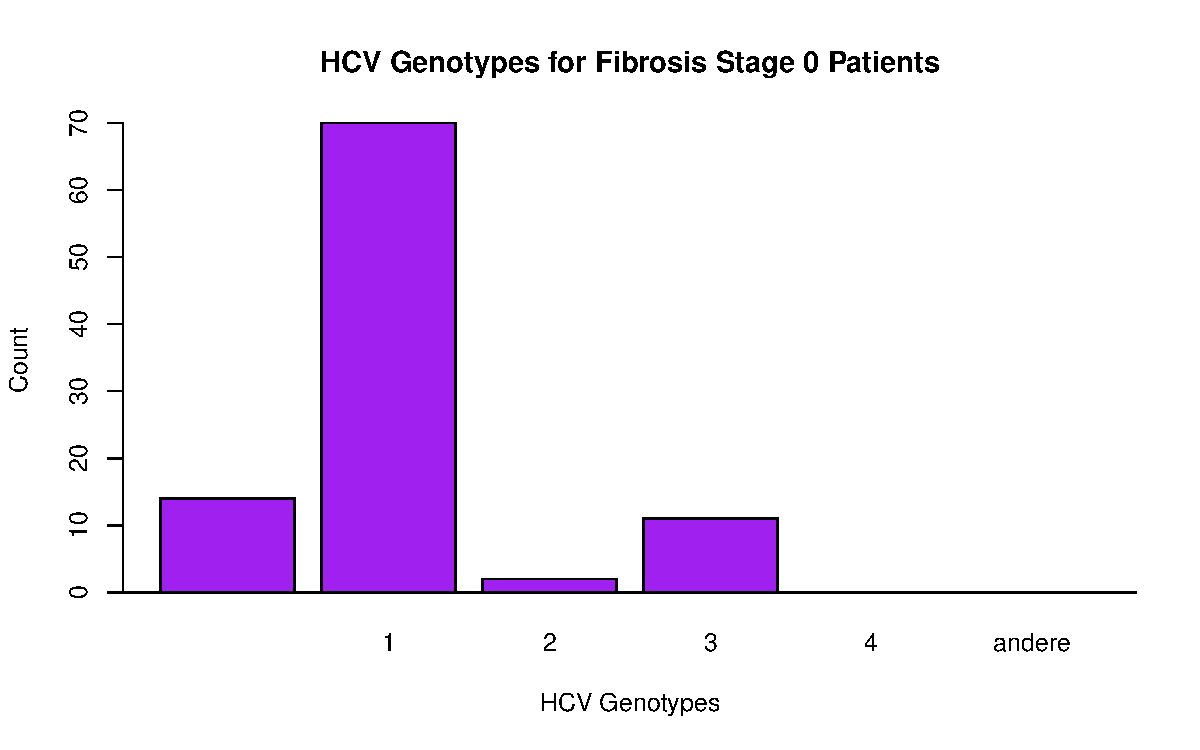
\includegraphics{HW0-025}

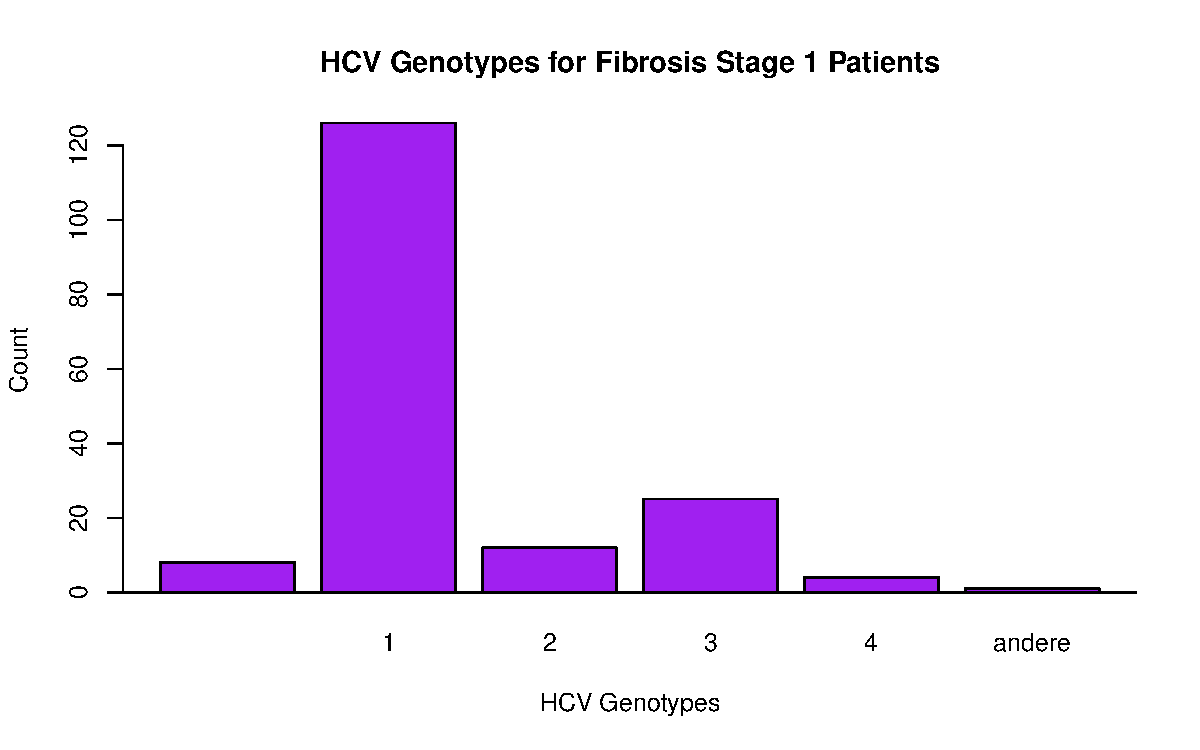
\includegraphics{HW0-026}

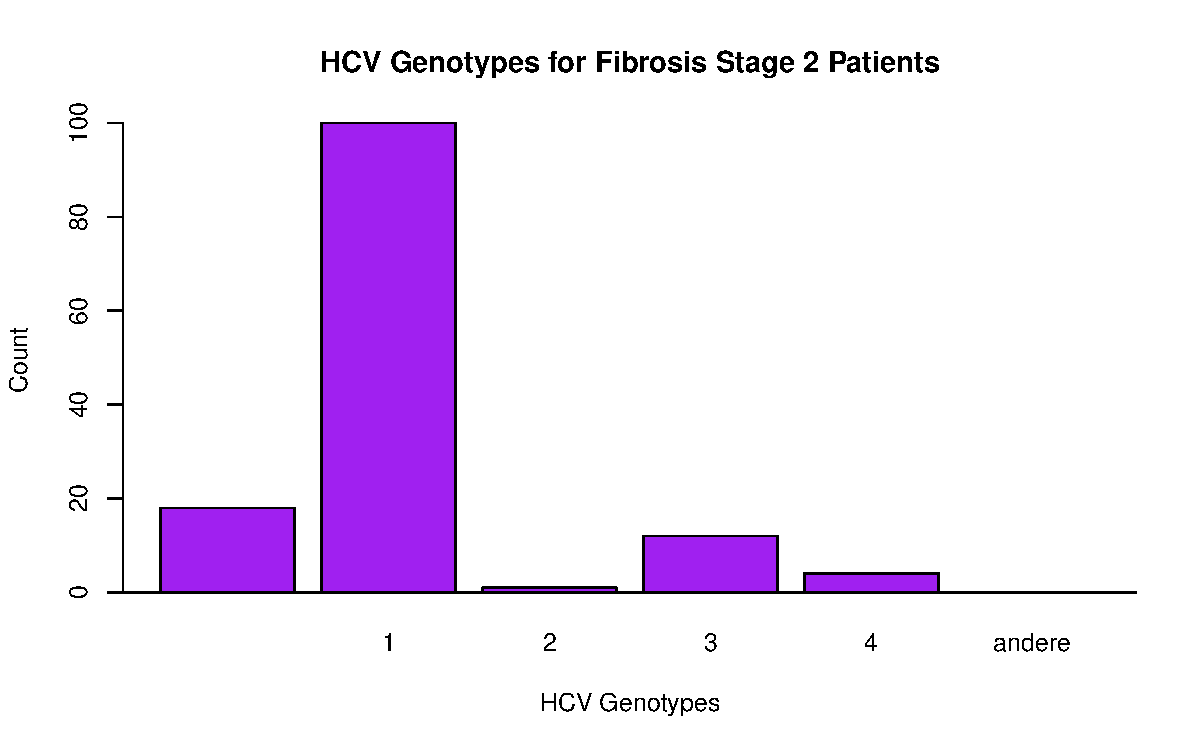
\includegraphics{HW0-027}

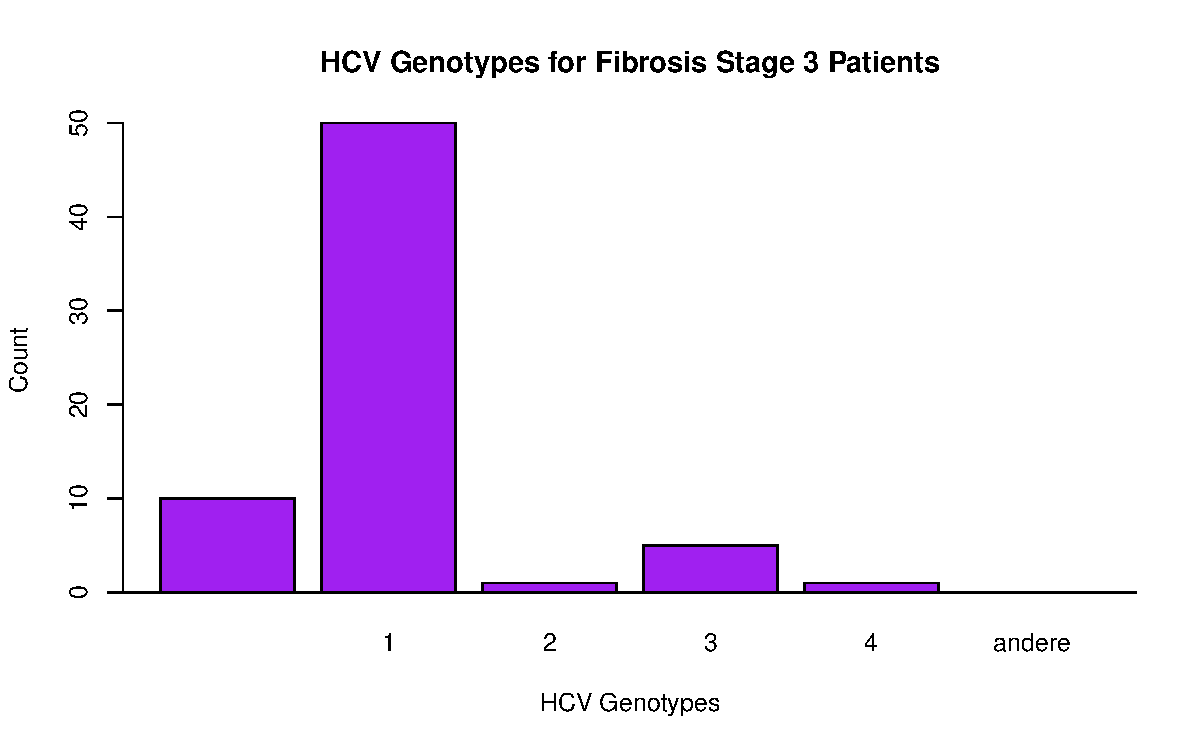
\includegraphics{HW0-028}

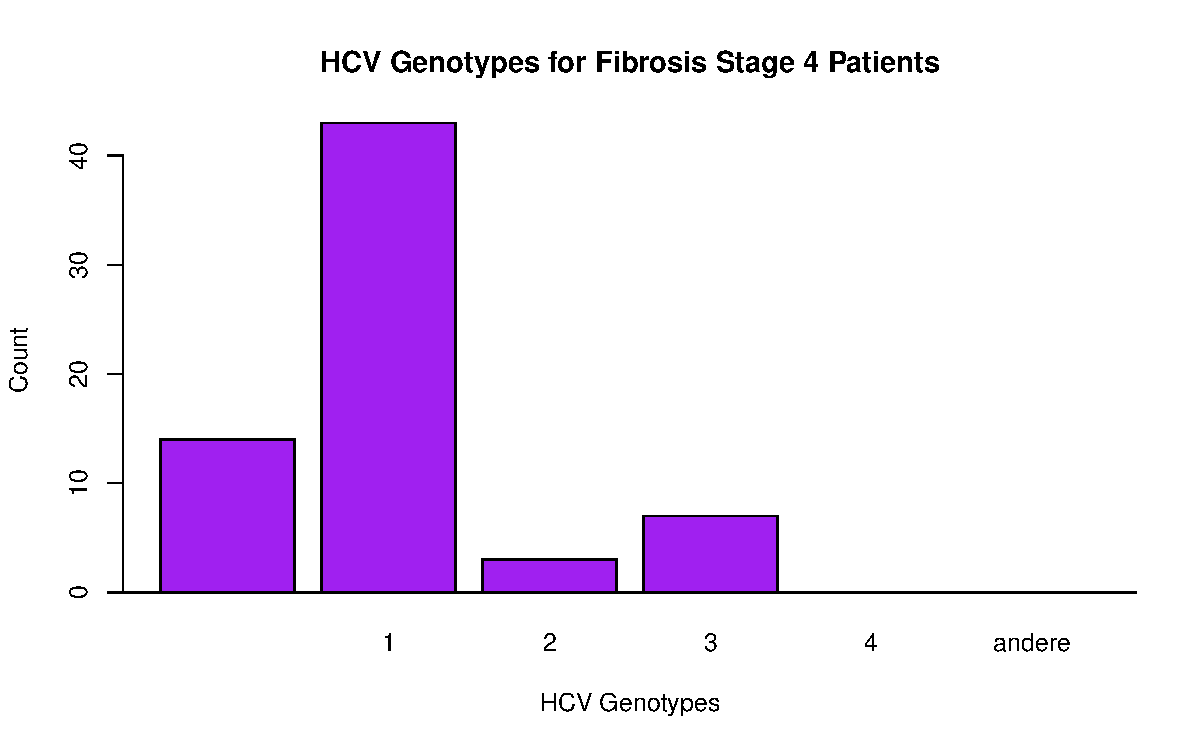
\includegraphics{HW0-029}

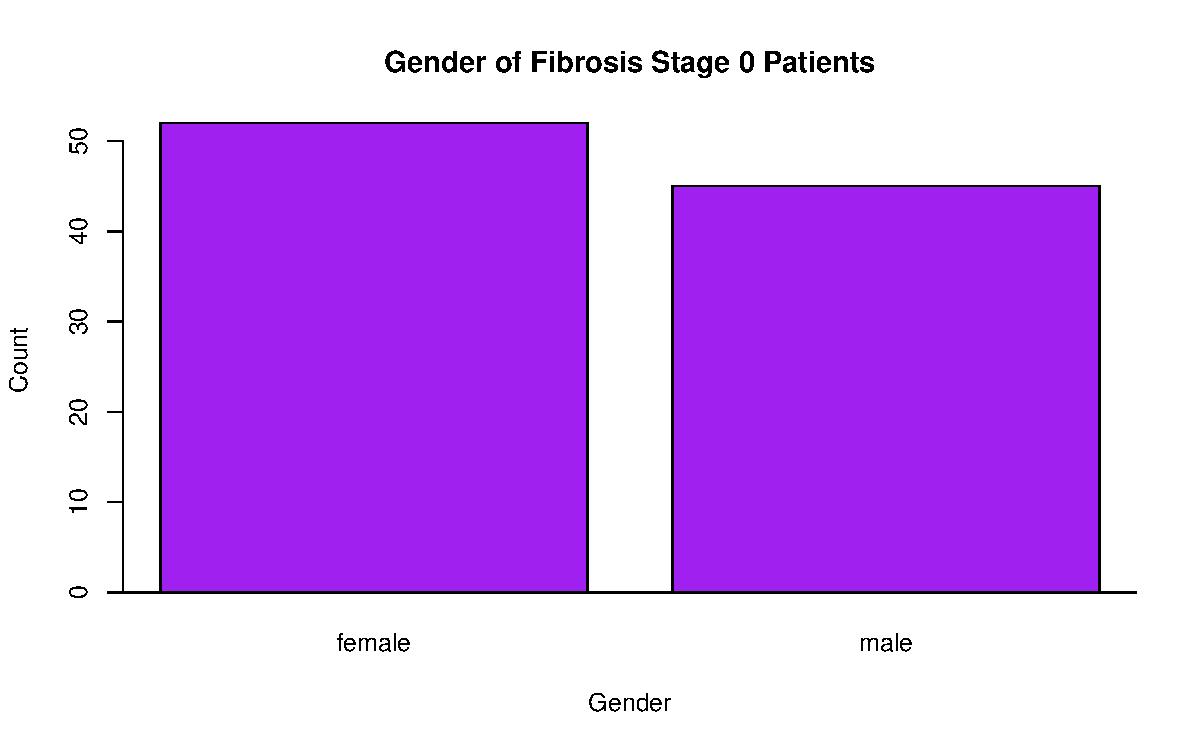
\includegraphics{HW0-030}

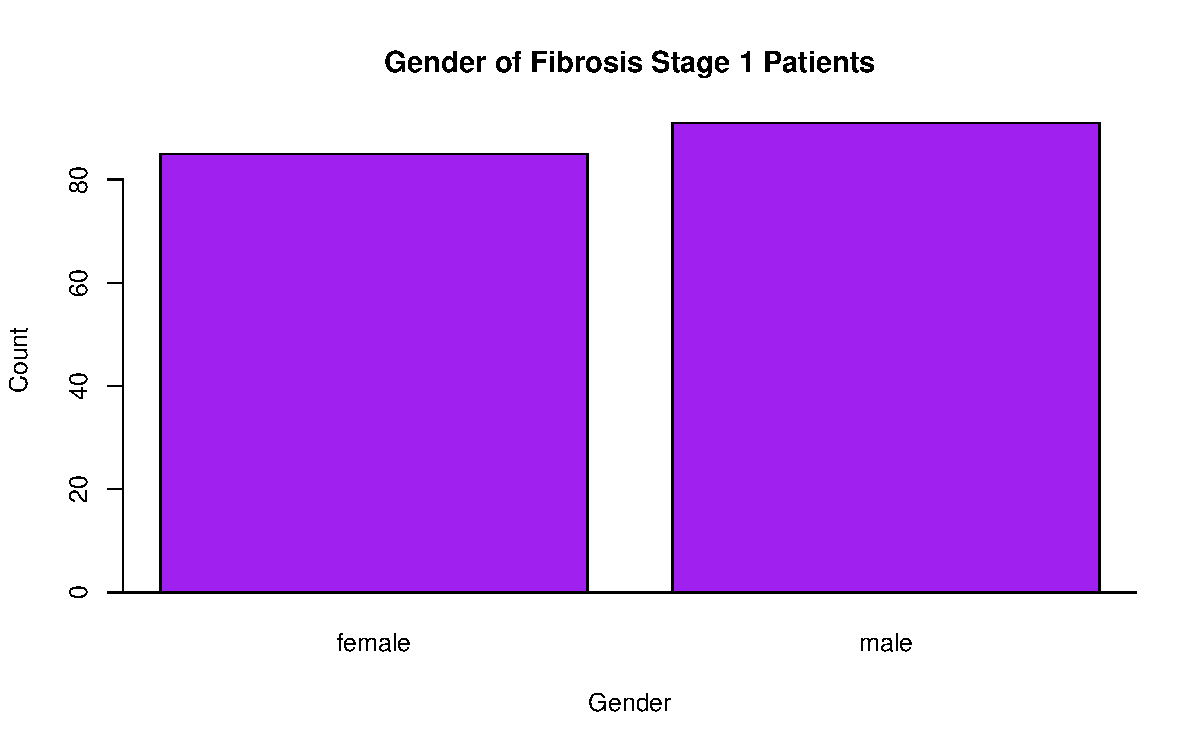
\includegraphics{HW0-031}

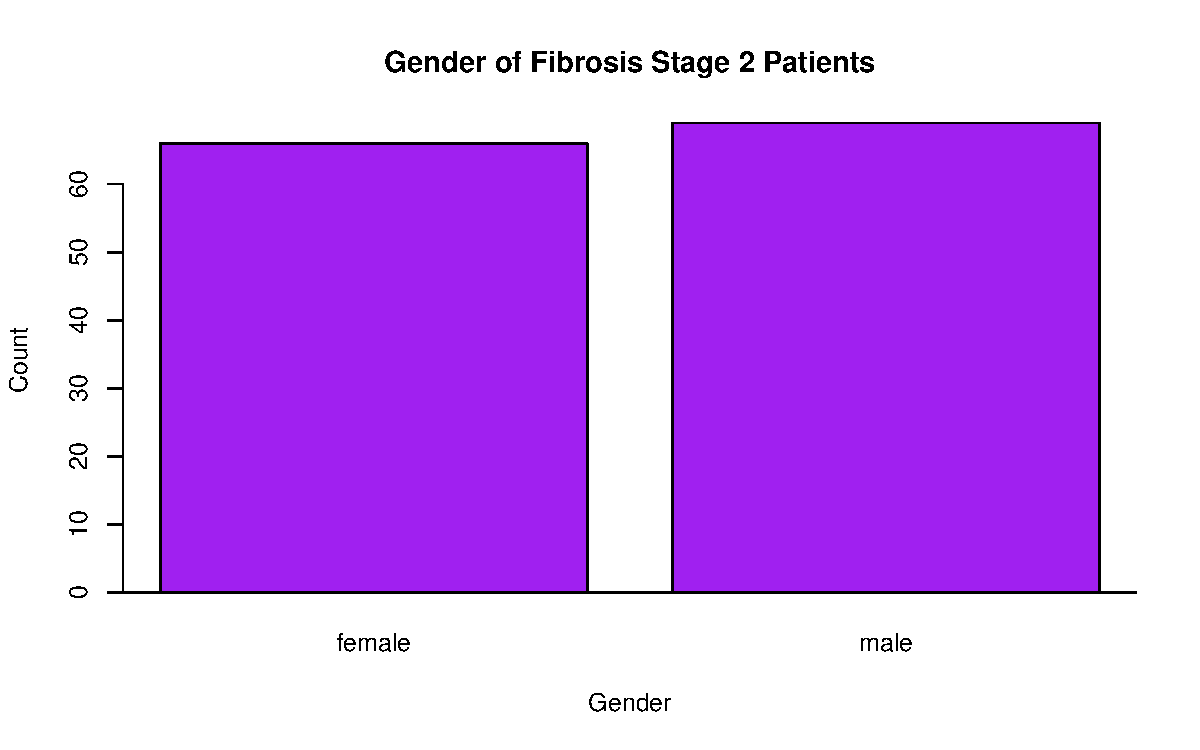
\includegraphics{HW0-032}

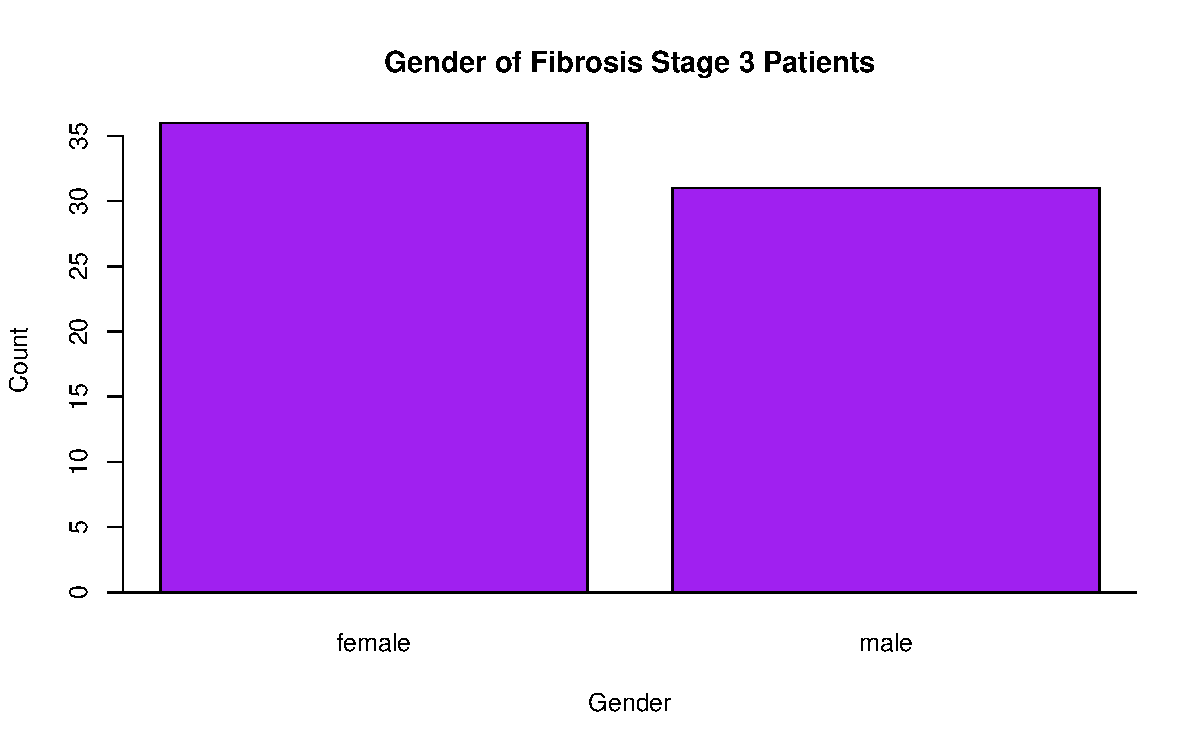
\includegraphics{HW0-033}

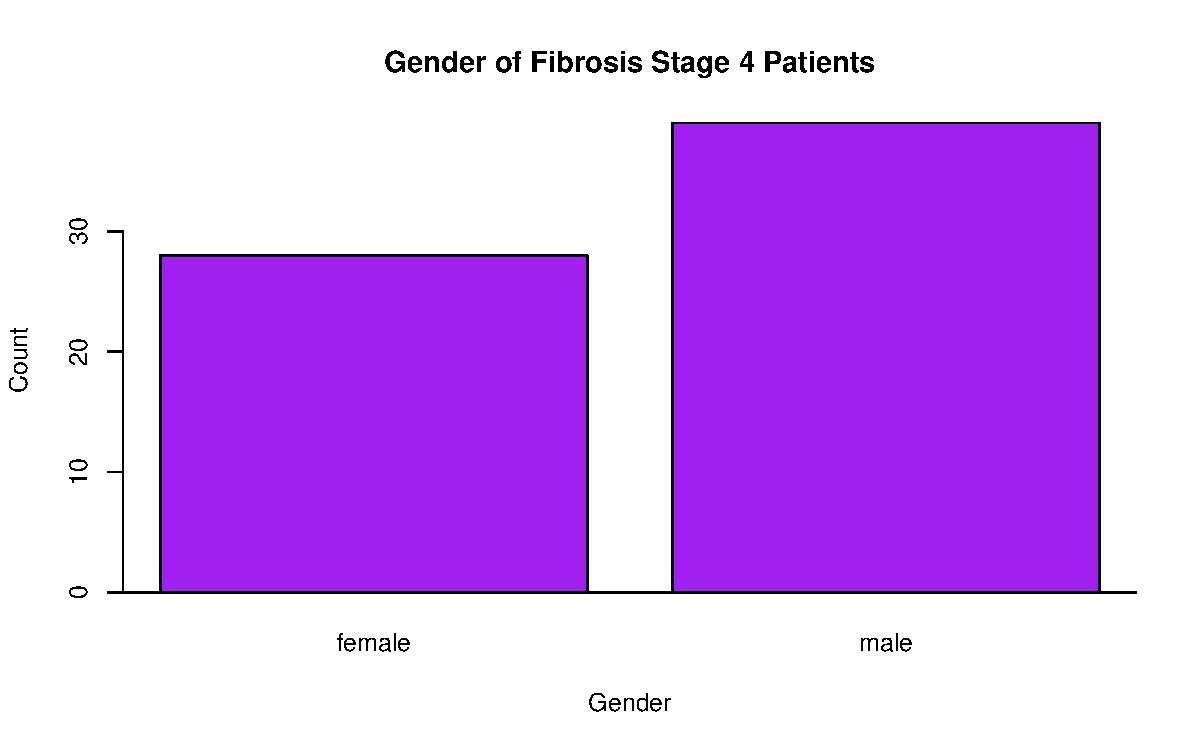
\includegraphics{HW0-034}
\newpage
\bibliography{bib}
\end{document}
